\section{ГЛАВА 6 ПРОЕКТИРОВАНИЕ ПОЛЬЗОВАТЕЛЬСКОГО ИНТЕРФЕЙСА МОБИЛЬНОГО ПРИЛОЖЕНИЯ}
На основе анализа требований, проведённого в предыдущей главе, сформированы функциональные приоритеты и целевые пользовательские сценарии. Учитывая разнообразие целевой аудитории — от студентов до пожилых пользователей и людей с ограниченными возможностями — разработка интуитивно понятного, доступного и адаптивного пользовательского интерфейса приобретает критически важное значение. В данной главе рассматриваются основные этапы проектирования интерфейсов, используемые подходы, технические требования и методология, применённая при создании макетов экранов мобильного приложения.
Целью главы является формирование целостного представления о структуре и логике интерфейсов до начала этапа разработки, что позволяет заранее выявить потенциальные проблемы, повысить удобство взаимодействия с приложением и сократить время на доработки в будущем.

\subsection*{Цели и задачи главы}
\begin{itemize}
    \item Определить основные принципы проектирования пользовательского интерфейса с учётом пользовательских историй и сценариев;
    \item Разработать макеты ключевых экранов мобильного приложения;
    \item Зафиксировать требования к элементам управления, визуальному стилю и адаптивности;
    \item Представить план работ по реализации интерфейсов;
    \item Построить диаграммы вариантов использования (use case diagrams) и активности (activity diagrams) для ключевых функций приложения.
\end{itemize}

\subsection*{Структура главы}
\begin{itemize}
    \item \textbf{2.1. Принципы и подходы к проектированию интерфейса} — описание используемых принципов UX/UI-дизайна, подходов к проектированию и обоснование выбора Flutter как инструмента реализации.
    \item \textbf{2.2. Разработка макетов интерфейса} — представление макетов ключевых экранов с комментариями к функциональным элементам, цветовой палитре и навигации.
    \item \textbf{2.3. Технические требования к интерфейсу} — спецификация требований к адаптивности, доступности, скорости отклика и другим техническим характеристикам UI.
    \item \textbf{2.4. Диаграммы вариантов использования и активности} — визуализация сценариев взаимодействия пользователей с приложением.
    \item \textbf{2.5. План реализации интерфейсов} — последовательность этапов разработки интерфейсов, включая создание компонентов, тестирование и возможные улучшения.
\end{itemize}

\subsection*{6.1. Принципы и подходы к проектированию интерфейса}
\addcontentsline{toc}{subsection}{6.1 Принципы и подходы к проектированию интерфейса}
Проектирование пользовательского интерфейса (UI) мобильного приложения осуществляется на основе современных принципов UX/UI-дизайна с учётом функциональных требований, определённых в результате анализа пользовательских историй. Основной задачей данного этапа является формирование логичной, интуитивной и визуально согласованной структуры взаимодействия пользователя с функциональными возможностями приложения.

\subsubsection*{Методология проектирования}
Для проектирования интерфейса использовалась итеративная модель разработки, предполагающая последовательное уточнение требований и постепенное усложнение макетов. Каждый экран и компонент интерфейса проектировался с учётом обратной связи от потенциальных пользователей и возможных ограничений платформы. Акцент был сделан на Mobile-First подход, что предполагает оптимизацию интерфейса в первую очередь под смартфоны как основное устройство использования.

\subsubsection*{Подход к организации интерфейса}
Архитектура интерфейса базируется на компонентной модели. Каждый экран приложения разбит на независимые компоненты, такие как панели фильтрации, карточки маршрутов, блоки навигации и другие элементы. Компонентный подход позволяет повторно использовать элементы интерфейса в разных частях приложения, упрощает тестирование и ускоряет разработку.
Организация экранов построена с применением навигационной модели «нижнее таб-меню + стековая навигация». Основные разделы приложения (поиск маршрутов, избранное, карта, профиль) доступны через нижнюю панель навигации, а переход между экранами внутри каждого раздела осуществляется по стековой модели. Это обеспечивает понятную логику перемещения между экранами и предсказуемость поведения приложения для пользователя.

\subsubsection*{Принципы UX/UI-дизайна}
Проектирование интерфейса базируется на следующих ключевых принципах:
\begin{itemize}
    \item Консистентность (consistency) — элементы управления, цвета, шрифты и отступы унифицированы по всему приложению, что способствует снижению когнитивной нагрузки.
    \item Принцип визуальной иерархии — важные элементы визуально выделяются с помощью цвета, размера и расположения. Это позволяет пользователю быстро ориентироваться в интерфейсе.
    \item Доступность (accessibility) — реализуемые интерфейсы адаптированы для пользователей с ограниченными возможностями. Используются крупные кликабельные области, читаемые шрифты, высококонтрастные элементы. В дальнейшем планируется реализация поддержки скринридеров.
    \item Адаптивность — интерфейс корректно отображается на различных размерах экранов (от малых смартфонов до планшетов) за счёт применения гибких сеток и пропорционального масштабирования элементов.
\end{itemize}

\subsubsection*{Выбор технологии реализации}
Для разработки пользовательского интерфейса выбрана кроссплатформенная технология Flutter, позволяющая создавать приложения под Android и iOS с единой кодовой базой. Основные причины выбора Flutter:
\begin{itemize}
    \item Высокая производительность благодаря нативной компиляции;
    \item Поддержка гибкой и настраиваемой системы пользовательских интерфейсов;
    \item Развитая экосистема готовых виджетов и библиотек;
    \item Возможность реализации сложной анимации и пользовательских сценариев с минимальными затратами ресурсов.
\end{itemize}
Использование Flutter позволяет ускорить процесс прототипирования и обеспечить визуальное соответствие макетов конечной реализации.

\subsubsection*{Прототипирование}
Прототипирование экранов проводилось с использованием Figma, что позволило визуализировать структуру будущего интерфейса, протестировать основные сценарии взаимодействия пользователей и согласовать макеты с участниками проектной команды до начала кодирования. На данном этапе были выявлены и скорректированы избыточные и неочевидные элементы навигации, обеспечив более чистую и логичную структуру приложения.

\subsection*{6.2. Разработка макетов интерфейса}
\addcontentsline{toc}{subsection}{6.2. Разработка макетов интерфейса}
Основываясь на выявленных пользовательских историях и функциональных требованиях, представленных в первой главе, настоящая глава посвящена проектированию интерфейсной части мобильного приложения для путешествий. Основной задачей данного этапа стало создание интуитивно понятного, функционального и универсального интерфейса, способного удовлетворить потребности различных категорий пользователей, включая молодёжь, семьи с детьми, пожилых людей, пользователей с ограниченными возможностями, тревел-блогеров и администраторов туристических сообществ.
Проектирование охватывает следующие ключевые аспекты: определение структуры экранов, визуальных макетов, технических требований к пользовательскому интерфейсу, а также анализ пользовательских сценариев с применением диаграмм прецедентов и активностей.

\subsubsection*{Требования к пользовательскому интерфейсу}
В процессе проектирования пользовательского интерфейса были выделены следующие технические и функциональные требования:
\begin{itemize}
    \item Кроссплатформенность: Приложение должно работать как на Android, так и на iOS-устройствах. В качестве фреймворка выбран Flutter, обеспечивающий единую кодовую базу.
    \item Доступность: Интерфейс должен учитывать потребности пользователей с ограниченными возможностями (поддержка экранных читалок, контрастные цвета, крупные элементы навигации).
    \item Производительность: Быстрая загрузка экранов, оптимизированные анимации, минимальное потребление ресурсов устройства.
    \item Масштабируемость: Интерфейс должен адаптироваться под экраны различных размеров, поддерживать горизонтальную и вертикальную ориентацию.
    \item Оффлайн-режим: Предусмотрена возможность загрузки маршрутов и карты для последующего использования без подключения к интернету.
    \item Персонализация: Пользовательский интерфейс должен предлагать индивидуальные рекомендации и учитывать предпочтения пользователя.
    \item Безопасность: Все действия, связанные с персональными данными (профиль, история маршрутов, комментарии), должны быть защищены механизмами аутентификации и авторизации.
\end{itemize}

\subsection*{6.3. Проектирование структуры экранов и пользовательских сценариев} 
\addcontentsline{toc}{subsection}{6.3. Проектирование структуры экранов и пользовательских сценариев}
Проектирование структуры экранов мобильного приложения выполнялось на основе предварительно собранных требований и пользовательских историй, проанализированных в первой главе. Основной целью данного этапа стало определение ключевых пользовательских сценариев, их последовательности и логики переходов между экранами.
Разработка структуры началась с выделения функциональных блоков, необходимых для реализации всех целевых сценариев использования. Были определены следующие основные группы экранов:
\begin{itemize}
    \item Главный экран: Шапка экрана содержит быстрый поиск маршрутов, персональные предложения, рекламные интеграции, категории маршрутов. Нижний прокручиваемый блок – персонально подобранные маршруты подобранные маршруты в виде ленты постов. (см. Рис.2.2.1.)
\end{itemize}
\begin{figure}[H]
        \centering
        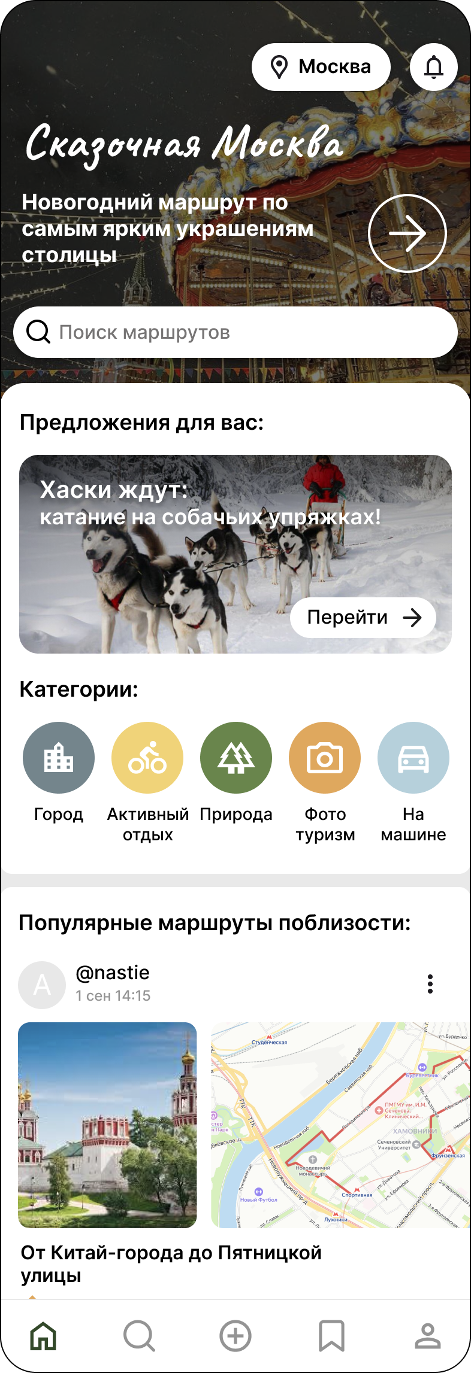
\includegraphics[width=0.4\linewidth]{Images/ui/Picture1.png}
        \caption{Главный экран}
        \label{fig:main_screen_ui_1}
\end{figure}

\begin{itemize}
    \item Экран поиска — предоставляет расширенные фильтры для подбора маршрутов по таким параметрам как расстояние и сложность. Также содержит быстрый поиск по категориям и местам поблизости с пользователем. (см. Рис. 2.2.2.-2.2.3.)
\end{itemize}
\begin{figure}[H]
        \centering
        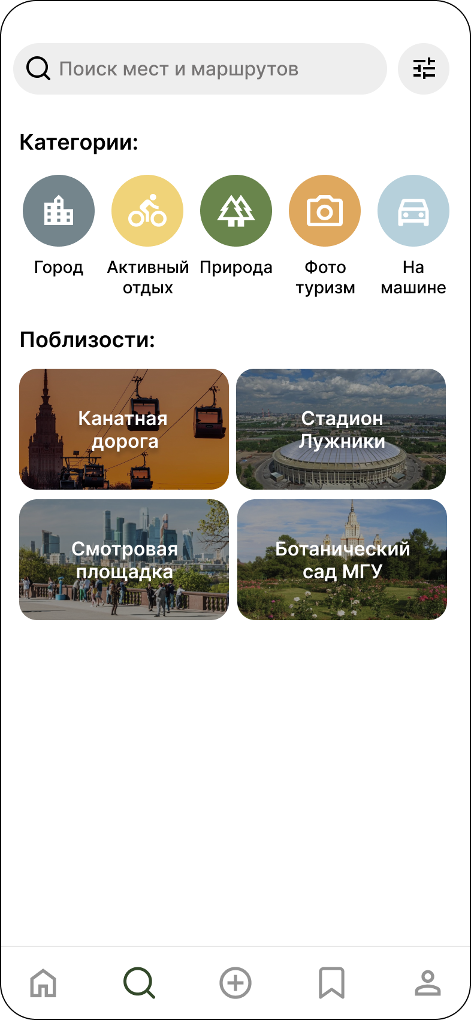
\includegraphics[width=0.4\linewidth]{Images/ui/Picture2.png}
        \caption{Экран поиска}
        \label{fig:ui_screen_2}
\end{figure}

\begin{figure}[H]
        \centering
        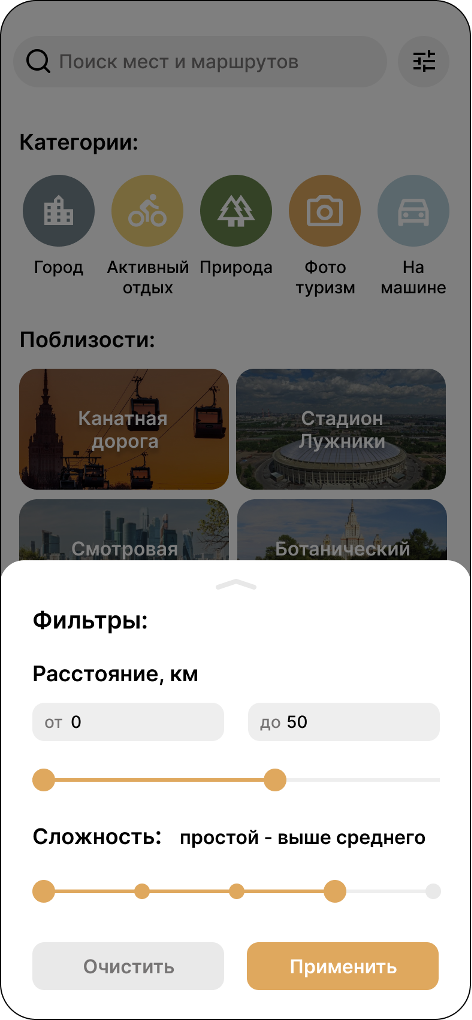
\includegraphics[width=0.4\linewidth]{Images/ui/Picture3.png}
        \caption{Окно с фильтрами на экране поиска}
        \label{fig:ui_screen_3}
\end{figure}
\begin{itemize}
    \item Экран маршрута — содержит карту и подробное описание маршрута. Имеет свернутый вид – с акцентом на карту и минимумом информации, и развернутый – содержит подробную информацию обо всех точках маршрута с описанием. (см. Рис. 2.2.4.-2.2.5.)
\end{itemize}
\begin{figure}[H]
        \centering
        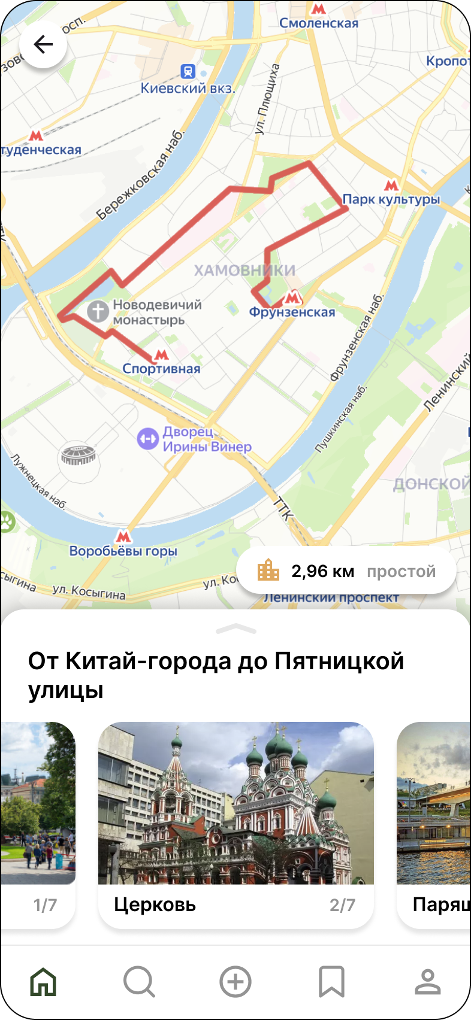
\includegraphics[width=0.4\linewidth]{Images/ui/Picture4.png}
        \caption{Экран просмотра маршрута}
        \label{fig:ui_screen_4}
\end{figure}

\begin{figure}[H]
        \centering
        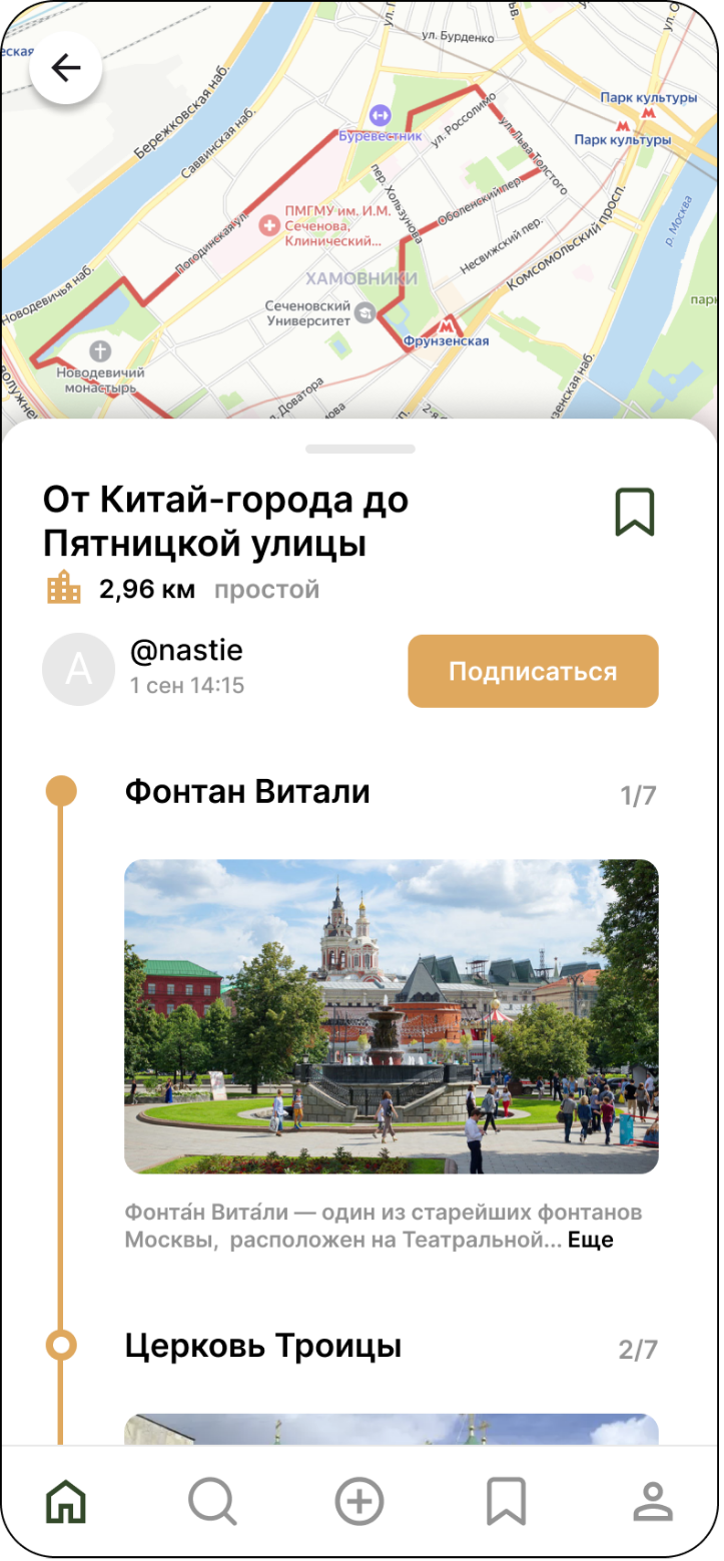
\includegraphics[width=0.4\linewidth]{Images/ui/Picture5.png}
        \caption{Развернутый вид экрана создания маршрута}
        \label{fig:ui_screen_5}
\end{figure}
\begin{itemize}
    \item Экраны создания маршрута. Процесс создания маршрута поделен на три экрана, чтобы не перегружать интерфейс. На первом экране пользователь задает название и выбирает категории маршрута. На втором экране доступен созданного обзор маршрута целиком. Третий экран дает возможность посмотреть маршрут на карте. (см. Рис. 2.2.6.-2.2.8.)
\end{itemize}
\begin{figure}[H]
        \centering
        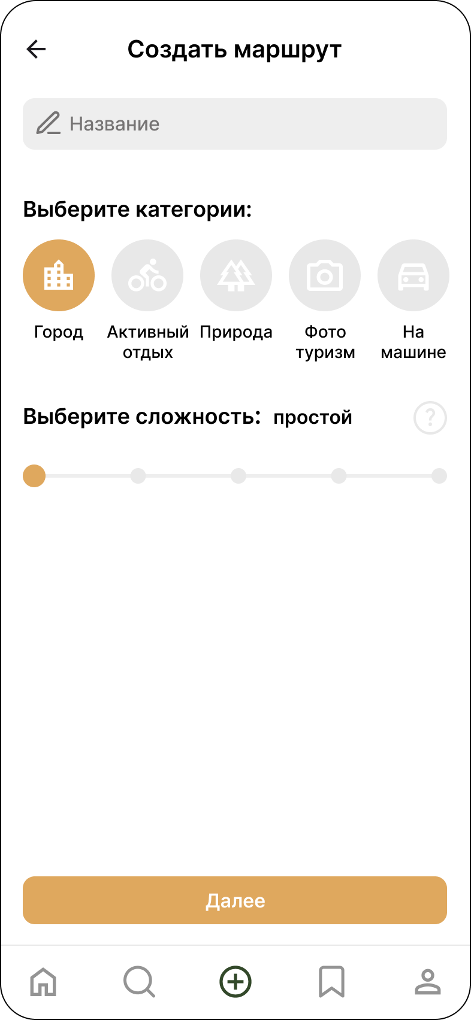
\includegraphics[width=0.4\linewidth]{Images/ui/Picture6.png}
        \caption{Экран создания маршрута. Первый этап}
        \label{fig:ui_screen_6}
\end{figure}
\begin{figure}[H]
        \centering
        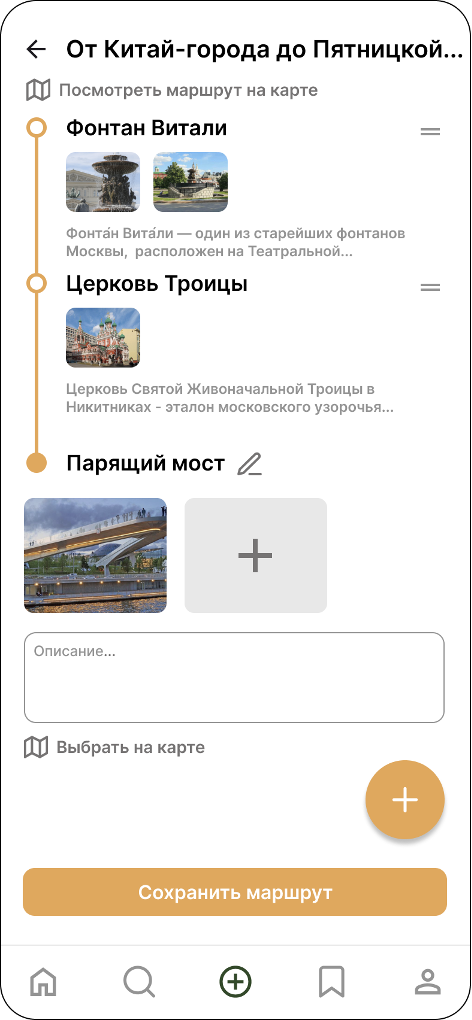
\includegraphics[width=0.4\linewidth]{Images/ui/Picture7.png}
        \caption{Экран создания маршрута. Второй этап}
        \label{fig:ui_screen_7}
\end{figure}

\begin{figure}[H]
        \centering
        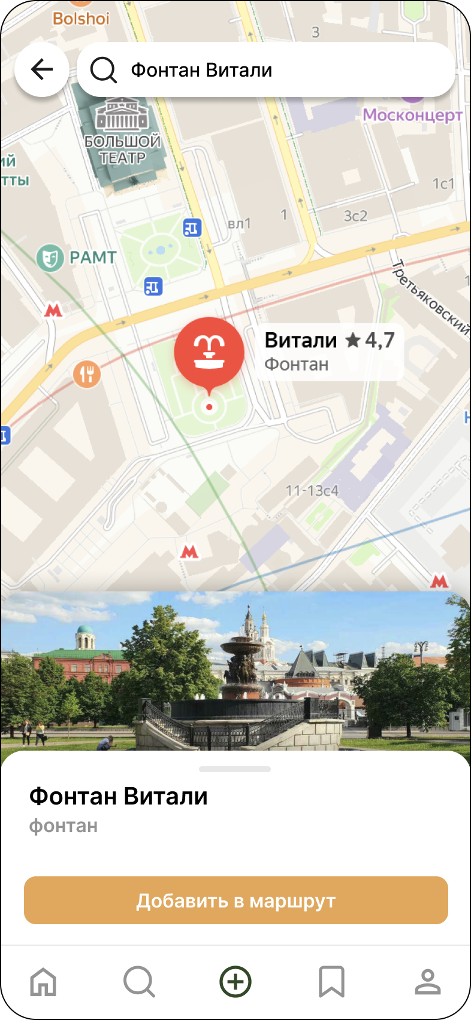
\includegraphics[width=0.4\linewidth]{Images/ui/Picture8.png}
        \caption{Экран выбора точки маршрута на карте}
        \label{fig:ui_screen_8}
\end{figure}

\begin{itemize}
    \item Профиль пользователя — включает историю активности, список избранных и созданных маршрутов. (см. Рис. 2.2.9.)
\end{itemize}
\begin{figure}[H]
        \centering
        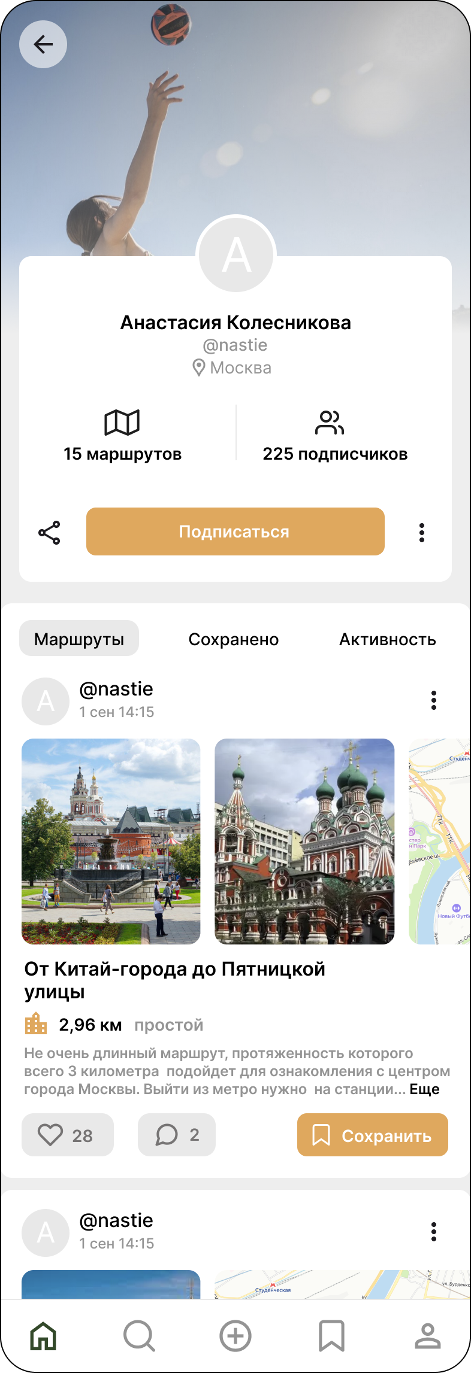
\includegraphics[width=0.4\linewidth]{Images/ui/Picture9.png}
        \caption{Экран профиля пользователя}
        \label{fig:ui_screen_9}
\end{figure}
Особое внимание при проектировании было уделено доступности интерфейса для различных категорий пользователей: людей с ограниченными возможностями, семей с детьми, пожилых пользователей и других. Это выразилось в адаптивной навигации, масштабируемости шрифтов, использовании контрастных цветов и возможности фильтрации контента по критериям доступности.
Каждый из экранов был детально проработан с учётом следующих аспектов:
\begin{itemize}
    \item последовательность пользовательских действий для достижения цели (например, планирование маршрута, добавление в избранное, просмотр отзывов);
    \item взаимодействие между экранами и логика переходов;
    \item минимизация числа шагов при выполнении частых сценариев;
    \item интуитивная организация интерфейса, соответствующая привычным шаблонам мобильных приложений.
\end{itemize}

\subsection*{6.4. Технические требования к интерфейсу}
\addcontentsline{toc}{subsection}{6.4. Технические требования к интерфейсу}
При проектировании пользовательского интерфейса были определены ключевые технические характеристики, необходимые для обеспечения стабильной, удобной и универсальной работы мобильного приложения. Эти требования охватывают аспекты адаптивности, доступности, отклика интерфейса, кроссплатформенности и других параметров, влияющих на пользовательский опыт.

\subsubsection*{Адаптивность и масштабируемость}
\begin{itemize}
    \item Интерфейс должен корректно отображаться на устройствах с различными размерами экранов (от смартфонов с диагональю 4 дюйма до планшетов с диагональю 12 дюймов).
    \item Используется система адаптивной вёрстки с применением MediaQuery, LayoutBuilder и Flexible/Expanded компонентов во Flutter.
    \item Все элементы интерфейса масштабируются в зависимости от плотности пикселей (pixel ratio), что обеспечивает корректную визуализацию на устройствах с высоким разрешением (Retina, AMOLED и т.д.).
\end{itemize}

\subsubsection*{Доступность (Accessibility)}
\begin{itemize}
    \item Приложение должно быть совместимо с системами экранного озвучивания (например, TalkBack и VoiceOver).
    \item Элементы управления снабжаются семантическими метками (Semantics, Tooltip, aria-label).
    \item Цветовая палитра и контрастность соответствуют рекомендациям WCAG 2.1 (уровень AA и выше).
    \item Минимальный размер интерактивных элементов — 48x48 dp, согласно рекомендациям Google.
    \item Навигация должна быть возможна как с помощью сенсорного ввода, так и с помощью вспомогательных технологий (переключатели, клавиатуры).
\end{itemize}

\subsubsection*{Производительность и скорость отклика}
\begin{itemize}
    \item Интерфейс должен обеспечивать отклик на действия пользователя в пределах 100 мс, приоритет на отсутствие «задержек» между взаимодействиями.
    \item Используется lazy-загрузка компонентов (ListView.builder, FutureBuilder) для экономии памяти и ускорения загрузки.
    \item Изображения и карты кэшируются и масштабируются под размер экрана для минимизации объёма загружаемых данных.
    \item Предусмотрена предварительная загрузка данных и отображение placeholder-компонентов для плавности восприятия.
\end{itemize}

\subsubsection*{Работа в офлайн-режиме}
\begin{itemize}
    \item Интерфейс должен предоставлять доступ к маршрутам, загруженным ранее, без подключения к интернету.
    \item Предусмотрены состояния online, offline и reconnecting, влияющие на доступность определённых функций.
    \item Компоненты синхронизируются с сервером при восстановлении подключения, с отображением индикаторов статуса.
\end{itemize}

\subsubsection*{Интерактивность и отклик на действия}
\begin{itemize}
    \item Все действия пользователя сопровождаются визуальной и/или тактильной обратной связью (нажатия, свайпы, ошибки).
    \item Предусмотрены состояния загрузки (loading), ошибки (error), успешного завершения действий (success) для всех ключевых операций.
\end{itemize}

\subsubsection*{Кроссплатформенность}
\begin{itemize}
    \item Приложение должно иметь идентичный набор функций и поведение на Android и iOS.
    \item Используются только те компоненты Flutter, которые обеспечивают корректную работу на обеих платформах.
    \item Сторонние библиотеки и плагины подбираются с учётом их поддержки в обеих системах.
\end{itemize}

\subsubsection*{Безопасность взаимодействия}
\begin{itemize}
    \item Обработка ошибок и недоступности функций реализована на уровне интерфейса — пользователь получает понятные уведомления и возможные пути решения (например, перезагрузить экран, проверить подключение).
\end{itemize}
